\documentclass[12pt]{article}
\usepackage[margin=2.5cm]{geometry}
\usepackage{enumerate}
\usepackage{amsfonts}
\usepackage{amsmath}
\usepackage{fancyhdr}
\usepackage{amsmath}
\usepackage{amssymb}
\usepackage{amsthm}
\usepackage{mdframed}
\usepackage{graphicx}
\usepackage{subcaption}
\usepackage{adjustbox}
\usepackage{listings}
\usepackage{xcolor}
\usepackage{booktabs}
\usepackage[utf]{kotex}
\usepackage{hyperref}

\definecolor{codegreen}{rgb}{0,0.6,0}
\definecolor{codegray}{rgb}{0.5,0.5,0.5}
\definecolor{codepurple}{rgb}{0.58,0,0.82}
\definecolor{backcolour}{rgb}{0.95,0.95,0.92}

\lstdefinestyle{mystyle}{
    backgroundcolor=\color{backcolour},
    commentstyle=\color{codegreen},
    keywordstyle=\color{magenta},
    numberstyle=\tiny\color{codegray},
    stringstyle=\color{codepurple},
    basicstyle=\ttfamily\footnotesize,
    breakatwhitespace=false,
    breaklines=true,
    captionpos=b,
    keepspaces=true,
    numbers=left,
    numbersep=5pt,
    showspaces=false,
    showstringspaces=false,
    showtabs=false,
    tabsize=1
}

\lstset{style=mystyle}

\pagestyle{fancy}
\renewcommand{\headrulewidth}{0.4pt}
\lhead{CSC 209}
\rhead{Review 4 Solution}

\begin{document}
\title{CSC 209 Review 4 Solution}
\maketitle

\bigskip

\begin{enumerate}[1.]
    \item

    The answer is \texttt{a) *p} and \texttt{g) *\&i}.

    \bigskip

    \underline{\textbf{Notes}}

    \bigskip

    \begin{itemize}
        \item \textbf{Address and Indirection Pointers}

        \begin{itemize}
            \item If \texttt{x} is a variable, \texttt{\&x} points to its memory address
            \item * in \texttt{*p} is called \textbf{Indirection operator}
            \begin{itemize}
                \item Allows variable to gain access to the object pointed by \texttt{p}
            \end{itemize}
        \end{itemize}
        \item \textbf{Aliases}

        \begin{itemize}
            \item Is the situation where the value in same memory location can be accessed using different variable names.

            \bigskip

            \underline{\textbf{Example 1:}}

            \bigskip

            \texttt{int i, p*;\\
            p = \& i;\\
            printf("\%d$\backslash$n", *p); /* *p is an alias of i */}

            \bigskip

            \underline{\textbf{Example 2:}}

            \bigskip

            \texttt{int i, p*;\\
            p = *\&i /* *p is an alias of i */}
        \end{itemize}
    \end{itemize}

    \item

    \bigskip

    The answers are \texttt{b) *p = \&i;}, \texttt{f) p = q;}, and \texttt{i) *p = *q;}

    \bigskip

    \begin{mdframed}
    \underline{\textbf{Correct Solution}}

    \bigskip

    The answers are \color{red}\texttt{e) p = *\&q;}\color{black}, \texttt{f) p = q;}, and \texttt{i) *p = *q;}

    \bigskip

    \color{red}\texttt{p = *\&q;} is the same as \texttt{p = q}\color{black}

    \end{mdframed}

    \underline{\textbf{Notes}}

    \begin{itemize}
        \item The \texttt{*} operator turns a \textit{value} of type \texttt{pointer to T} into a \textit{variable} of type \texttt{T}.
        \item The \texttt{\&} operator turns a \textit{variable} of type \texttt{T} into a \textit{value} of type pointer to \texttt{T}.
        \item \textbf{Pointer Assignment}

        \begin{itemize}
            \item The following is an example of correct pointer assignment

            \bigskip

            \texttt{int i, j, *p. *q;\\
            p = \&i;
            }

            \bigskip

            \begin{itemize}
                \item Means the memory address of \texttt{p} is pointing to memory address of \texttt{i}
            \end{itemize}

            \bigskip

            \item The following is another valid example of pointer assignment

            \bigskip

            \texttt{int i, j, *p. *q;\\
            p = \&i;\\
            q = p;
            }

            \bigskip

            \begin{itemize}
                \item Means memory address of \texttt{q} is the memory address of \texttt{p} (which is the memory address of \texttt{i})
            \end{itemize}

            \begin{center}
            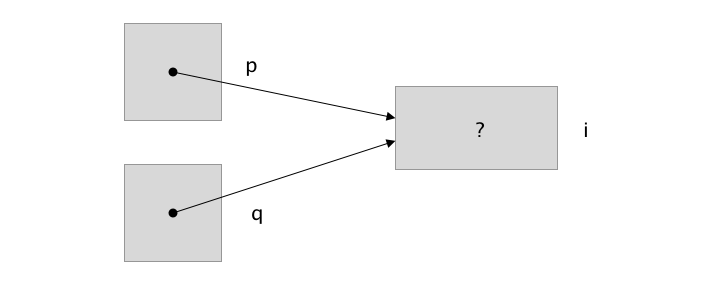
\includegraphics[width=0.6\linewidth]{images/review_4_solution_1.png}
            \end{center}

            \bigskip

            \texttt{*p = 1;}

            \begin{center}
            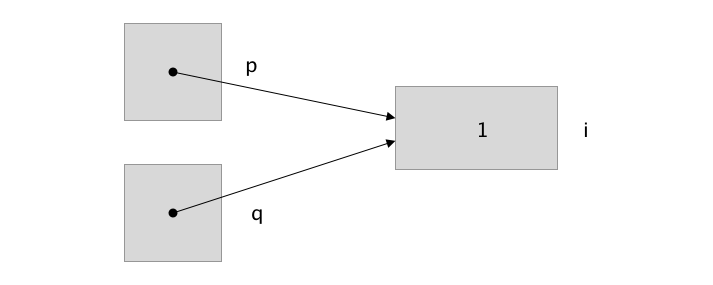
\includegraphics[width=0.6\linewidth]{images/review_4_solution_2.png}
            \end{center}

            \bigskip

            \texttt{*p = 2;}

            \begin{center}
            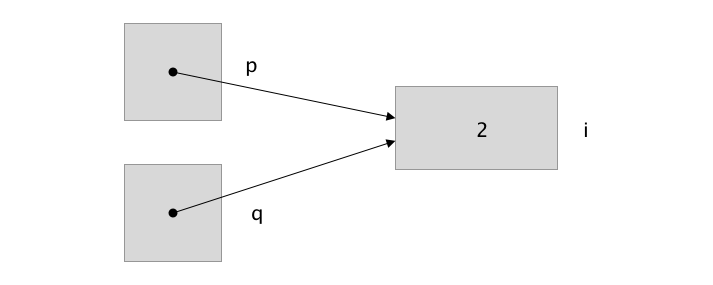
\includegraphics[width=0.6\linewidth]{images/review_4_solution_3.png}
            \end{center}

            \item The following is not a pointer assignment

            \bigskip

            \texttt{*q = *p}

            \begin{itemize}
                \item It \underline{copies the value that} \texttt{p} points to
            \end{itemize}

            \begin{center}
            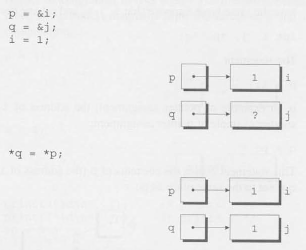
\includegraphics[width=0.6\linewidth]{images/review_4_solution_4.png}
            \end{center}

        \end{itemize}
    \end{itemize}
\end{enumerate}

\end{document}